\documentclass{article}
\usepackage[margin=1in]{geometry}
\usepackage{amsmath,amsthm,amssymb}
\usepackage{bbm,enumerate,mathtools}
\usepackage{tikz,pgfplots}
\usepackage{chessboard}
\usepackage[hidelinks]{hyperref}
\usepackage{multicol} % Problem 35

\newenvironment{question}{\begin{trivlist}\item[\textbf{Question.}]}{\end{trivlist}}
\newenvironment{note}{\begin{trivlist}\item[\textbf{Note.}]}{\end{trivlist}}
\newenvironment{references}{\begin{trivlist}\item[\textbf{References.}]}{\end{trivlist}}
\newenvironment{related}{\begin{trivlist}\item[\textbf{Related.}]\end{trivlist}\begin{enumerate}}{\end{enumerate}}


\begin{document}
Suppose you are given an $n \times m$ grid, and I then think of a rectangle with
its corners on grid points.
I then ask you to ``black out'' as many of the gridpoints as possible,
in such a way that you can still guess my rectangle after I tell you all of the
non-blacked out vertices that its corners lie on.\\
\begin{figure}[!h]
  \centering
  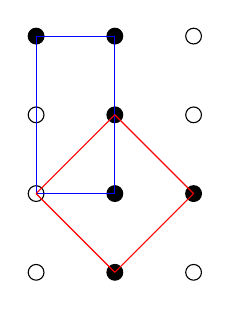
\begin{tikzpicture}
    \foreach \x in {1,...,3}
    \foreach \y in {1,...,4}
    {
      \draw (\x,\y) circle (0.1cm);
    }
    \fill (1,4) circle (0.1cm); \fill (2,4) circle (0.1cm);
                                \fill (2,3) circle (0.1cm);
                                \fill (2,2) circle (0.1cm); \fill (3,2) circle (0.1cm);
                                \fill (2,1) circle (0.1cm);

    \draw[blue] (1,3) -- (1,4);
    \draw[blue] (1,2) -- (1,3);
    \draw[blue] (2,3) -- (2,4);
    \draw[blue] (2,2) -- (2,3);
    \draw[blue] (1,4) -- (2,4);
    \draw[blue] (1,2) -- (2,2);

    \draw[red] (1, 2) -- (2, 3);
    \draw[red] (2, 3) -- (3, 2);
    \draw[red] (3, 2) -- (2, 1);
    \draw[red] (2, 1) -- (1, 2);
  \end{tikzpicture}
  \caption{
    An example of an invalid ``black out'' for an $3 \times 4$ grid.
    The blue rectangle and the red rectangle have the same presentation.
  }
\end{figure}

\begin{question}
  How many vertices may be crossed out such that every rectangle can still
    be uniquely identified?
\end{question}
\begin{related}
  \item What if the interior of the rectangle is lit up instead?
  \item What if all gridpoints that instersect the perimeter are lit up?
  \item What if the rectangles must be square?
  \item What if parallelogams are used instead of rectangles?
  \item What if the rectangles must be horizontal or vertical?
  \item What if the rectangles must be horizontal, vertical, or 45° diagonal?
  \item What if this is done on a triangular grid with equilateral triangles?
  \item What if this is done in more dimensions
    (e.g. with a rectangular prism or tetrahedron?)
\end{related}
\end{document}
